\chapter{Kombinatoriikka}

Kombinatoriikka tarkoittaa yhdistelmien määrän laskemista.
Tavoitteena on yleensä laskea yhdistelmät
tehokkaasti niin, että jokaista yhdistelmää
ei tarvitse muodostaa erikseen, vaan yhdistelmien määrän
saa selville hyödyntämällä säännöllisyyksiä ja
dynaamista ohjelmointia.

\section{Perustekniikat}

\subsubsection{Summat ja tulot}

Summa kertoo yhdistelmien määrän,
kun on olemassa useita vaihtoehtoja
ja niistä valitaan yksi.
Tulo kertoo puolestaan yhdistelmien määrän,
kun tehdään joukko peräkkäisiä valintoja.

\begin{task}
Ravintolassa A on 4 alkuruokaa,
7 pääruokaa ja 3 jälkiruokaa.
Ravintolassa B on 6 alkuruokaa,
8 pääruokaa ja 2 jälkiruokaa.
Montako menua on olemassa (alkuruoka, pääruoka, jälkiruoka)?
\end{task}

Ravintolassa A menuja on $4 \cdot 7 \cdot 3 = 84$
ja ravintolassa B menuja on $6 \cdot 8 \cdot 2 = 96$.
Niinpä menuja on yhteensä $84+96=180$.

\subsubsection{Merkkijonot}

On $k^n$ tapaa muodostaa $n$ merkin pituinen merkkijono,
kun käytössä on $k$ merkkiä,
koska jokaisessa merkkijonon kohdassa merkin valintaan
on $k$ vaihtoehtoa.
Esimerkiksi on $2^3=8$ tapaa muodostaa kolmen merkin pituinen
bittijono:
000, 001, 010, 011, 100, 101, 110 ja 111.

\subsubsection{Permutaatiot}

Kertoma $n!$ ilmaisee, monellako tavalla voidaan
järjestää $n$ alkiota
eli muodostaa $n$ alkion permutaatio.
Tämä perustuu siihen, että ensimmäisen
alkion voi valita $n$ tavalla,
seuraavan $n-1$ tavalla, jne.
Esimerkiksi merkkijonolla \texttt{abc} on
$3!=6$ permutaatiota:
\texttt{abc},
\texttt{acb},
\texttt{bac},
\texttt{bca},
\texttt{cab} ja
\texttt{cba}.

\subsubsection{Rekursio}

Kombinatorisen tehtävän ratkaisun voi usein esittää
rekursiivisena funktiona.
Tämän jälkeen ratkaisun voi laskea tehokkaasti
dynaamisella ohjelmoinnilla.
Näin on esimerkiksi seuraavassa tehtävässä:

\begin{task}
Monellako tavalla luvun $n$ voi esittää positiivisten
kokonaislukujen summana?
Esimerkiksi luvun 4 voi esittää 8 tavalla:
$1+1+1+1$, $1+1+2$, $1+2+1$, $2+1+1$,
$2+2$, $3+1$, $1+3$ ja $4$.
\end{task}

Merkitään $f(n)$:llä esitystapojen määrää luvulle $n$,
eli esimerkiksi $f(4)=8$.
Funktion voi laskea rekursiivisesti seuraavasti:
\begin{equation*}
    f(n) = \begin{cases}
               1               & n = 0\\
               f(0)+f(1)+\ldots+f(n-1) & n > 0\\
           \end{cases}
\end{equation*}
Seuraava koodi muodostaa dynaamisen ohjelmoinnin avulla
taulukon \texttt{d}, jossa $\texttt{d}[k]=f(k)$,
kun $k=0,1,\ldots,n$:
\begin{lstlisting}
d[0] = 1;
for (int i = 1; i <= n; i++) {
    for (int j = 0; j < n; j++) {
        d[i] += d[j];
    }
}
\end{lstlisting}

\section{Binomikerroin}

Binomikerroin ${n \choose k}$ ilmaisee,
monellako tavalla $n$ alkion joukosta
voidaan muodostaa $k$ alkion osajoukko.
Esimerkiksi ${5 \choose 2}=10$,
koska alkioista $\{A,B,C,D,E\}$
voidaan valita $10$ tavalla $2$ alkiota:
\[ \{A,B\}, \{A,C\}, \{A,D\}, \{A,E\}, \{B,C\}, 
\{B,D\}, \{B,E\}, \{C,D\}, \{C,E\}, \{D,E\} \]

\subsubsection{Laskutapa 1}

Binomikertoimen voi laskea rekursiivisesti seuraavasti:

\[
{n \choose k}  =  {n-1 \choose k-1} + {n-1 \choose k}
\]

Ideana rekursiossa on tarkastella tiettyä
joukon alkiota $x$.
Jos alkio $x$ valitaan osajoukkoon,
täytyy vielä valita $n-1$ alkiosta $k-1$ alkiota.
Jos taas alkiota $x$ ei valita osajoukkoon,
täytyy vielä valita $n-1$ alkiosta $k$ alkiota.

Rekursion pohjatapaukset ovat seuraavat:

\[
{n \choose 0}  =  {n \choose n} = 1
\]

Selityksenä on, että on aina yksi tapa
muodostaa tyhjä osajoukko,
samoin kuin valita kaikki alkiot osajoukkoon.

\subsubsection{Laskutapa 2}

Toinen tapa laskea binomikerroin on seuraava:
\[
{n \choose k}  =  \frac{n!}{k!(n-k)!}.
\]
Kaavassa $n!$ on $n$ alkion permutaatioiden määrä.
Ideana on käydä läpi kaikki permutaatiot
ja valita kussakin tapauksessa
permutaation $k$ ensimmäistä alkiota osajoukkoon.
Koska ei ole merkitystä,
missä järjestyksessä osajoukon alkiot
ja ulkopuoliset alkiot ovat,
tulos jaetaan luvuilla $k!$ ja $(n-k)!$.

\subsubsection{Ominaisuuksia}

Binomikertoimelle pätee
\[
{n \choose k}  =  {n \choose n-k},
\]
koska $k$ alkion valinta osajoukkoon
tarkoittaa samaa kuin että valitaan
$n-k$ alkiota osajoukon ulkopuolelle.

Binomikerrointen summa on
\[
{n \choose 0}+{n \choose 1}+{n \choose 2}+\ldots+{n \choose n}=2^n.
\]

Nimi ''binomikerroin'' tulee siitä, että

\[ (a+b)^n =
{n \choose 0} a^n b^0 + 
{n \choose 1} a^{n-1} b^1 +
\ldots + 
{n \choose n-1} a^1 b^{n-1} +
{n \choose n} a^0 b^n. \]
Binomikertoimet esiintyvät myös Pascalin
kolmiossa, jonka reunoilla on lukua 1
ja jokainen luku saadaan
kahden yllä olevan luvun summana:
\begin{center}
\begin{tikzpicture}{0.9}
\node at (0,0) {1};
\node at (-0.5,-0.5) {1};
\node at (0.5,-0.5) {1};
\node at (-1,-1) {1};
\node at (0,-1) {2};
\node at (1,-1) {1};
\node at (-1.5,-1.5) {1};
\node at (-0.5,-1.5) {3};
\node at (0.5,-1.5) {3};
\node at (1.5,-1.5) {1};
\node at (-2,-2) {1};
\node at (-1,-2) {4};
\node at (0,-2) {6};
\node at (1,-2) {4};
\node at (2,-2) {1};
\node at (-2,-2.5) {$\ldots$};
\node at (-1,-2.5) {$\ldots$};
\node at (0,-2.5) {$\ldots$};
\node at (1,-2.5) {$\ldots$};
\node at (2,-2.5) {$\ldots$};
\end{tikzpicture}
\end{center}

\subsubsection{Laatikot ja pallot}

Laatikot ja pallot on usein hyödyllinen malli
kombinatoriikan tehtävissä.
Siinä $n$ laatikkoon sijoitetaan $k$ palloa.
Tarkastellaan seuraavaksi kolmea tapausta:

\textit{Tapaus 1}: Kuhunkin laatikkoon saa sijoittaa
enintään yhden pallon.
Esimerkiksi kun $n=5$ ja $k=2$,
sijoitustapoja on 10:

\begin{center}
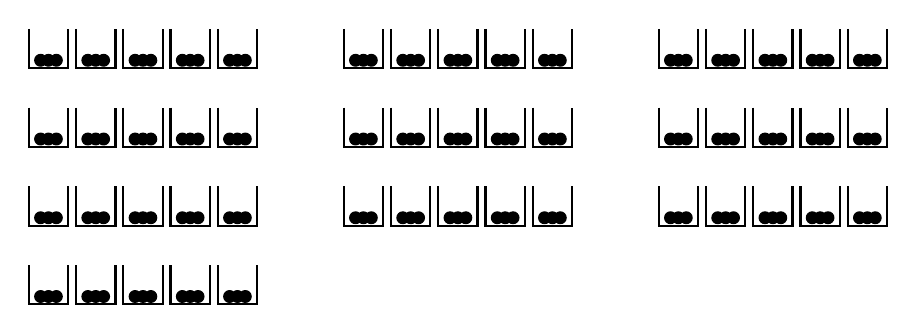
\begin{tikzpicture}[scale=0.5]
\newcommand\lax[3]{
\path[draw,thick,-] (#1-0.5,#2+0.5) -- (#1-0.5,#2-0.5) --
                    (#1+0.5,#2-0.5) -- (#1+0.5,#2+0.5);
\ifthenelse{\equal{#3}{1}}{\draw[fill=black] (#1,#2-0.3) circle (0.15);}{}
\ifthenelse{\equal{#3}{2}}{\draw[fill=black] (#1-0.2,#2-0.3) circle (0.15);}{}
\ifthenelse{\equal{#3}{2}}{\draw[fill=black] (#1+0.2,#2-0.3) circle (0.15);}{}
}
\newcommand\laa[7]{
    \lax{#1}{#2}{#3}
    \lax{#1+1.2}{#2}{#4}
    \lax{#1+2.4}{#2}{#5}
    \lax{#1+3.6}{#2}{#6}
    \lax{#1+4.8}{#2}{#7}
}

\laa{0}{0}{1}{1}{0}{0}{0}
\laa{0}{-2}{1}{0}{1}{0}{0}
\laa{0}{-4}{1}{0}{0}{1}{0}
\laa{0}{-6}{1}{0}{0}{0}{1}
\laa{8}{0}{0}{1}{1}{0}{0}
\laa{8}{-2}{0}{1}{0}{1}{0}
\laa{8}{-4}{0}{1}{0}{0}{1}
\laa{16}{0}{0}{0}{1}{1}{0}
\laa{16}{-2}{0}{0}{1}{0}{1}
\laa{16}{-4}{0}{0}{0}{1}{1}

\end{tikzpicture}
\end{center}

Tässä tapauksessa vastauksen kertoo suoraan binomikerroin ${n \choose k}$.

\textit{Tapaus 2}: Samaan laatikkoon saa sijoittaa
monta palloa.
Esimerkiksi kun $n=5$ ja $k=2$, sijoitustapoja on 15:

\begin{center}
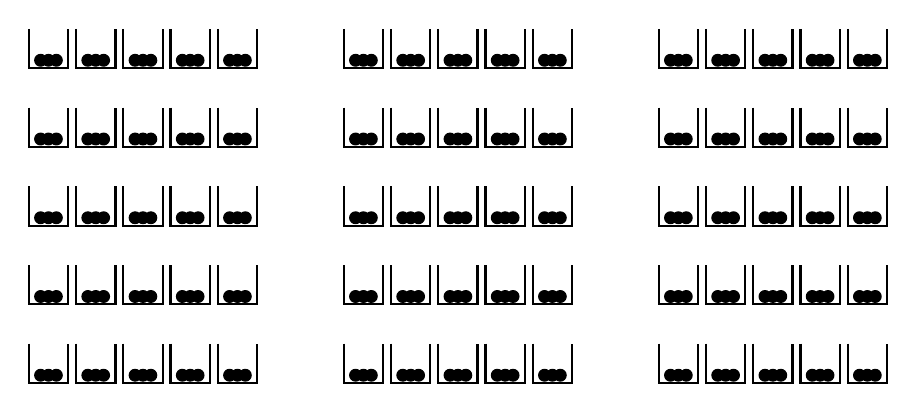
\begin{tikzpicture}[scale=0.5]
\newcommand\lax[3]{
\path[draw,thick,-] (#1-0.5,#2+0.5) -- (#1-0.5,#2-0.5) --
                    (#1+0.5,#2-0.5) -- (#1+0.5,#2+0.5);
\ifthenelse{\equal{#3}{1}}{\draw[fill=black] (#1,#2-0.3) circle (0.15);}{}
\ifthenelse{\equal{#3}{2}}{\draw[fill=black] (#1-0.2,#2-0.3) circle (0.15);}{}
\ifthenelse{\equal{#3}{2}}{\draw[fill=black] (#1+0.2,#2-0.3) circle (0.15);}{}
}
\newcommand\laa[7]{
    \lax{#1}{#2}{#3}
    \lax{#1+1.2}{#2}{#4}
    \lax{#1+2.4}{#2}{#5}
    \lax{#1+3.6}{#2}{#6}
    \lax{#1+4.8}{#2}{#7}
}

\laa{0}{0}{2}{0}{0}{0}{0}
\laa{0}{-2}{1}{1}{0}{0}{0}
\laa{0}{-4}{1}{0}{1}{0}{0}
\laa{0}{-6}{1}{0}{0}{1}{0}
\laa{0}{-8}{1}{0}{0}{0}{1}
\laa{8}{0}{0}{2}{0}{0}{0}
\laa{8}{-2}{0}{1}{1}{0}{0}
\laa{8}{-4}{0}{1}{0}{1}{0}
\laa{8}{-6}{0}{1}{0}{0}{1}
\laa{8}{-8}{0}{0}{2}{0}{0}
\laa{16}{0}{0}{0}{1}{1}{0}
\laa{16}{-2}{0}{0}{1}{0}{1}
\laa{16}{-4}{0}{0}{0}{2}{0}
\laa{16}{-6}{0}{0}{0}{1}{1}
\laa{16}{-8}{0}{0}{0}{0}{2}

\end{tikzpicture}
\end{center}

Prosessin voi kuvata merkkijonona, joka muodostuu
merkeistä ''o'' ja ''$\rightarrow$''.
Pallojen sijoittaminen alkaa
vasemmanpuoleisimmasta laatikosta.
Merkki ''o'' tarkoittaa, että pallo sijoitetaan
nykyiseen laatikkoon, ja merkki
''$\rightarrow$'' tarkoittaa, että siirrytään
seuraavaan laatikkoon.

Nyt jokainen sijoitustapa on merkkijono, jossa
on $k$ kertaa merkki ''o'' ja $n-1$ kertaa
merkki ''$\rightarrow$''.
Esimerkiksi sijoitustapaa
ylhäällä oikealla
vastaa merkkijono ''$\rightarrow$ $\rightarrow$ o $\rightarrow$ o $\rightarrow$''.
Niinpä sijoitustapojen määrä on ${n+k-1 \choose k}$.

\textit{Tapaus 3}: Kuhunkin laatikkoon saa sijoittaa
enintään yhden pallon ja lisäksi missään kahdessa
vierekkäisessä laatikossa ei saa olla palloa.
Esimerkiksi kun $n=5$ ja $k=2$, sijoitustapoja on 6:


\begin{center}
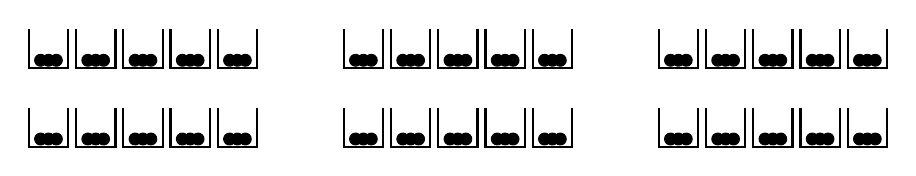
\begin{tikzpicture}[scale=0.5]
\newcommand\lax[3]{
\path[draw,thick,-] (#1-0.5,#2+0.5) -- (#1-0.5,#2-0.5) --
                    (#1+0.5,#2-0.5) -- (#1+0.5,#2+0.5);
\ifthenelse{\equal{#3}{1}}{\draw[fill=black] (#1,#2-0.3) circle (0.15);}{}
\ifthenelse{\equal{#3}{2}}{\draw[fill=black] (#1-0.2,#2-0.3) circle (0.15);}{}
\ifthenelse{\equal{#3}{2}}{\draw[fill=black] (#1+0.2,#2-0.3) circle (0.15);}{}
}
\newcommand\laa[7]{
    \lax{#1}{#2}{#3}
    \lax{#1+1.2}{#2}{#4}
    \lax{#1+2.4}{#2}{#5}
    \lax{#1+3.6}{#2}{#6}
    \lax{#1+4.8}{#2}{#7}
}

\laa{0}{0}{1}{0}{1}{0}{0}
\laa{0}{-2}{1}{0}{0}{1}{0}
\laa{8}{0}{1}{0}{0}{0}{1}
\laa{8}{-2}{0}{1}{0}{1}{0}
\laa{16}{0}{0}{1}{0}{0}{1}
\laa{16}{-2}{0}{0}{1}{0}{1}
\end{tikzpicture}
\end{center}

Tässä tapauksessa voi ajatella, että alussa $k$ palloa
ovat laatikoissaan ja joka välissä on yksi tyhjä laatikko.
Tämän jälkeen jää valittavaksi $n-k-(k-1)=n-2k+1$ tyhjän laatikon paikat.
Mahdollisia välejä on $k+1$, joten tapauksen 2 perusteella
sijoitustapoja on ${k+1+n-2k+1-1 \choose n-2k+1} = {n-k+1 \choose n-2k+1}$.

\subsubsection{Multinomikerroin}

Binomikertoimen yleistys on multinomikerroin

\[ {n \choose k_1,k_2,\ldots,k_m} = \frac{n!}{k_1! k_2! \cdots k_m!}, \]

missä $k_1+k_2+\cdots+k_m=n$.
Multinomikerroin ilmaisee, monellako tavalla $n$ alkiota voidaan jakaa osajoukkoihin,
joiden koot ovat $k_1,k_2,\ldots,k_m$.
Jos $m=2$, multinomikertoimen kaava vastaa binomikertoimen kaavaa.

\section{Catalanin luvut}

Catalanin luku $C_n$ ilmaisee,
montako tapaa on muodostaa kelvollinen sulkulauseke
$n$ alkusulusta ja $n$ loppusulusta.
Esimerkiksi $C_3=5$, koska 3 alkusulusta
ja 3 loppusulusta voidaan muodostaa
kelvolliset sulkulausekkeet
\texttt{()()()}, \texttt{(())()},
\texttt{()(())}, \texttt{((()))} ja \texttt{(()())}.

\subsubsection{Sulkulausekkeet}

Sulkulauseke on kelvollinen,
jos sitä vastaa jokin
matemaattinen lauseke,
josta on poistettu
kaikki merkit sulkuja lukuun ottamatta.
Esimerkiksi yllä mainittu sulkulauseke \texttt{(())()}
on kelvollinen, koska sitä vastaa
esimerkiksi matemaattinen lauseke $(2 \cdot (4+5)+3)\cdot(1+3)$.

Kelvollisen sulkulausekkeen voi tunnistaa käymällä
läpi lausekkeen merkit vasemmalta oikealle ja
pitämällä yllä laskuria, jonka arvo on aluksi 0.
Merkki \texttt{(} kasvattaa laskuria ja
merkki \texttt{)} vähentää laskuria.
Sulkulauseke on kelvollinen, jos laskurin arvo
on aina vähintään 0 ja lopuksi tarkalleen 0.

Huomaa myös, että kelvollisen sulkulausekkeen
jokaisessa alkuosassa alkusulkujen määrä on
sama tai suurempi kuin loppusulkujen määrä.

\subsubsection{Laskutapa 1}

Catalanin lukuja voi laskea rekursiivisesti seuraavasti:
\[ C_n = \sum_{i=0}^{n-1} C_{i} C_{n-i-1}\]
Summa käy läpi tavat
jakaa sulkulauseke kahteen osaan niin,
että kumpikin osa on kelvollinen sulkulauseke
ja alkuosa on mahdollisimman lyhyt mutta ei tyhjä.
Kunkin vaihtoehdon kohdalla alkuosassa
on $i+1$ sulkuparia ja lausekkeiden määrä
saadaan kertomalla keskenään:

\begin{itemize}
\item $C_{i}$: tavat muodostaa sulkulauseke
alkuosan sulkupareista ulointa sulkuparia lukuun ottamatta
\item $C_{n-i-1}$: tavat muodostaa sulkulauseke
loppuosan sulkupareista
\end{itemize}
Lisäksi pohjatapauksena on $C_0=1$, koska 0
sulkuparista voi muodostaa
tyhjän sulkulausekkeen.

\subsubsection{Laskutapa 2}

Catalanin lukuja voi laskea myös binomikertoimen avulla:
\[ C_n = \frac{1}{n+1} {2n \choose n}. \]
Kaavan voi perustella seuraavasti:

Kun käytössä on $n$ alkusulkua ja $n$ loppusulkua,
niistä voi muodostaa kaikkiaan ${2n \choose n}$
sulkulauseketta.
Lasketaan seuraavaksi, moniko tällainen
sulkulauseke \textit{ei} ole kelvollinen.

Jos sulkulauseke ei ole kelvollinen,
siinä on oltava alkuosa,
jossa loppusulkuja on alkusulkuja enemmän.
Muutetaan jokainen tällaisen alkuosan
sulkumerkki käänteiseksi.
Esimerkiksi lausekkeessa \texttt{())()(}
alkuosa on \texttt{())} ja kääntämisen
jälkeen lausekkeesta tulee \texttt{)((()(}.

Tuloksena olevassa lausekkeessa on $n+1$ alkusulkua
ja $n-1$ loppusulkua. Tällaisia lausekkeita on
kaikkiaan ${2n \choose n+1}$,
joka on sama kuin ei-kelvollisten
sulkulausekkeiden määrä.
Niinpä kelvollisten
sulkulausekkeiden määrä voidaan laskea kaavalla
\[{2n \choose n}-{2n \choose n+1} = {2n \choose n} - \frac{n}{n+1} {2n \choose n} = \frac{1}{n+1} {2n \choose n}.\]

\subsubsection{Binääripuut}

Toinen tulkinta Catalanin luvuille on,
että $C_n$ on $n$ alkion binääripuiden määrä.
Tässä tapauksessa summa
\[ C_n = \sum_{i=0}^{n-1} C_{i} C_{n-i-1},\]
käy läpi tavat muodostaa vasen ja oikea alipuu.
Kaavassa $i$ on vasemman alipuun koko ja 
$n-i-1$ on oikean alipuun koko.

Esimerkiksi $C_3=5$ ja vastaavat binääripuut ovat:

\begin{center}
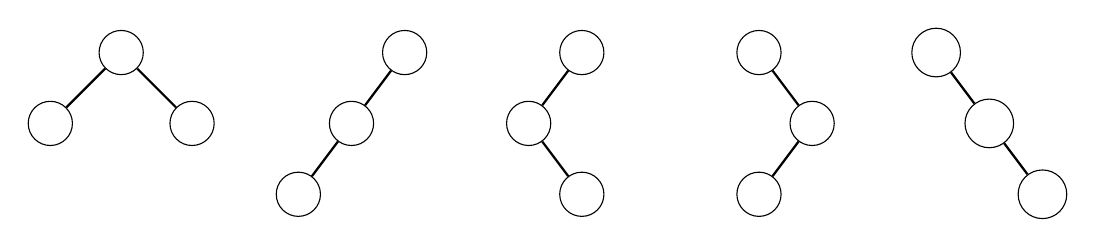
\begin{tikzpicture}[scale=0.9]
\node[draw, circle] (a1) at (0,0) {\phantom{o}};
\node[draw, circle] (a2) at (-1,-1) {\phantom{o}};
\node[draw, circle] (a3) at (1,-1) {\phantom{o}};
\path[draw,thick,-] (a1) -- (a2);
\path[draw,thick,-] (a1) -- (a3);

\node[draw, circle] (b1) at (4,0) {\phantom{o}};
\node[draw, circle] (b2) at (4-0.75,-1) {\phantom{o}};
\node[draw, circle] (b3) at (4-1.5,-2) {\phantom{o}};
\path[draw,thick,-] (b1) -- (b2);
\path[draw,thick,-] (b2) -- (b3);

\node[draw, circle] (c1) at (6.5,0) {\phantom{o}};
\node[draw, circle] (c2) at (6.5-0.75,-1) {\phantom{o}};
\node[draw, circle] (c3) at (6.5-0,-2) {\phantom{o}};
\path[draw,thick,-] (c1) -- (c2);
\path[draw,thick,-] (c2) -- (c3);

\node[draw, circle] (d1) at (9,0) {\phantom{o}};
\node[draw, circle] (d2) at (9+0.75,-1) {\phantom{o}};
\node[draw, circle] (d3) at (9-0,-2) {\phantom{o}};
\path[draw,thick,-] (d1) -- (d2);
\path[draw,thick,-] (d2) -- (d3);

\node[draw, circle] (e1) at (11.5,0) {\phantom{0}};
\node[draw, circle] (e2) at (11.5+0.75,-1) {\phantom{0}};
\node[draw, circle] (e3) at (11.5+1.5,-2) {\phantom{0}};
\path[draw,thick,-] (e1) -- (e2);
\path[draw,thick,-] (e2) -- (e3);
\end{tikzpicture}
\end{center}


\section{Inkluusio-ekskluusio}

Inkluusio-ekskluusio
on tekniikka, jonka avulla pystyy laskemaan
joukkojen yhdisteen koon leikkausten
kokojen perusteella ja päinvastoin.
Yksinkertainen esimerkki periaatteesta on kaava
\[ |A \cup B| = |A| + |B| - |A \cap B|,\]
jossa $A$ ja $B$ ovat joukkoja ja $|X|$
tarkoittaa joukon $X$ kokoa.
Seuraava kuva havainnollistaa kaavaa,
kun joukot ovat tason ympyröitä:

\begin{center}
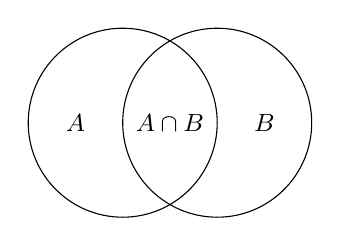
\begin{tikzpicture}[scale=0.8]

\draw (0,0) circle (1.5);
\draw (1.5,0) circle (1.5);

\node at (-0.75,0) {\small $A$};
\node at (2.25,0) {\small $B$};
\node at (0.75,0) {\small $A \cap B$};

\end{tikzpicture}
\end{center}

Tavoitteena on laskea, kuinka suuri on yhdiste $A \cup B$
eli alue, joka on toisen tai kummankin ympyrän sisällä.
Kuvan mukaisesti yhdisteen $A \cup B$ koko
saadaan laskemalla ensin yhteen ympyröiden $A$ ja $B$ koot
ja vähentämällä siitä sitten leikkauksen $A \cap B$ koko.

Samaa ideaa voi soveltaa, kun joukkoja on enemmän.
Kolmen joukon tapauksessa kaavasta tulee
\[ |A \cup B \cup C| = |A| + |B| + |C| - |A \cap B|  - |A \cap C|  - |B \cap C| + |A \cap B \cap C| \]
ja vastaava kuva on

\begin{center}
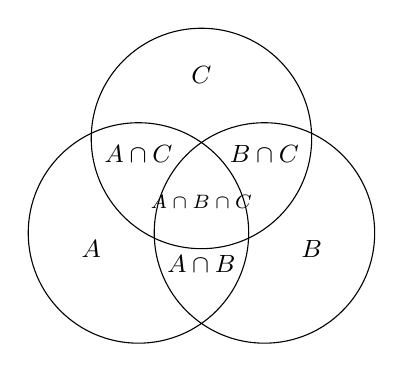
\begin{tikzpicture}[scale=0.8]

\draw (0,0) circle (1.75);
\draw (2,0) circle (1.75);
\draw (1,1.5) circle (1.75);

\node at (-0.75,-0.25) {\small $A$};
\node at (2.75,-0.25) {\small $B$};
\node at (1,2.5) {\small $C$};
\node at (1,-0.5) {\small $A \cap B$};
\node at (0,1.25) {\small $A \cap C$};
\node at (2,1.25) {\small $B \cap C$};
\node at (1,0.5) {\scriptsize $A \cap B \cap C$};

\end{tikzpicture}
\end{center}

Yleisessä tapauksessa yhdisteen $X_1 \cup X_2 \cup \cdots \cup X_n$
koon saa laskettua käymällä läpi kaikki tavat muodostaa
leikkaus joukoista $X_1,X_2,\ldots,X_n$.
Parittoman määrän joukkoja sisältävät leikkaukset
lasketaan mukaan positiivisina ja
parillisen määrän negatiivisina.

Huomaa, että vastaavat kaavat toimivat myös käänteisesti
leikkauksen koon laskemiseen yhdisteiden kokojen perusteella.
Esimerkiksi

\[ |A \cap B| = |A| + |B| - |A \cup B|\]

ja
\[ |A \cap B \cap C| = |A| + |B| + |C| - |A \cup B|  - |A \cup C|  - |B \cup C| + |A \cup B \cup C| .\]

\subsubsection{Esimerkki}

Tarkastellaan esimerkkinä seuraavaa tehtävää:

\begin{task}
Lukujonon $(1,2,\ldots,n)$
\textit{epäjärjestys} on permutaatio,
jossa mikään luku ei ole alkuperäisellä paikallaan.
Tehtäväsi on laskea, montako epäjärjestystä on olemasassa.
Esimerkiksi jos $n=3$, niin epäjärjestyksiä on kaksi: $(2,3,1)$ ja $(3,1,2)$
\end{task}

Yksi tapa lähestyä tehtävää on käyttää inkluusio-ekskluusiota.
Olkoon joukko $X_k$ niiden permutaatioiden joukko,
jossa kohdassa $k$ on luku $k$.
Esimerkiksi jos $n=3$, niin joukot ovat seuraavat:
\[
\begin{array}{lcl}
X_1 & = & \{(1,2,3),(1,3,2)\} \\
X_2 & = & \{(1,2,3),(3,2,1)\} \\
X_3 & = & \{(1,2,3),(2,1,3)\} \\
\end{array}
\]
Näitä joukkoja käyttäen epäjärjestysten määrä on
\[ n! - |X_1 \cup X_2 \cup \cdots \cup X_n|, \]
eli
riittää laskea joukkojen yhdisteen koko.
Tämä palautuu inkluusio-eks\-kluu\-sion avulla
joukkojen leikkausten kokojen laskemiseen,
mikä onnistuu tehokkaasti.
Esimerkiksi kun $n=3$, joukon $|X_1 \cup X_2 \cup X_3|$ koko on
\[
\begin{array}{lcl}
 & & |X_1| + |X_2| + |X_3| - |X_1 \cap X_2|  - |X_1 \cap X_3|  - |X_2 \cap X_3| + |X_1 \cap X_2 \cap X_3| \\
 & = & 2+2+2-1-1-1+1 \\
 & = & 4, \\
\end{array}
\]
joten ratkaisujen määrä on $3!-4=2$.

Osoittautuu, että tehtävän voi ratkaista myös toisella
tavalla käyttämättä inkluusio-ekskluusiota.
Merkitään $f(n)$:llä jonon $(1,2,\ldots,n)$ epäjärjestysten määrää,
jolloin seuraava rekursio pätee:

\begin{equation*}
    f(n) = \begin{cases}
               0               & n = 1\\
               1               & n = 2\\
               (n-1)(f(n-2) + f(n-1)) & n>2 \\
           \end{cases}
\end{equation*}

Kaavan voi perustella käymällä läpi tapaukset,
miten luku 1 muuttuu epäjärjestyksessä.
On $n-1$ tapaa valita jokin luku $x$ luvun 1 tilalle.
Jokaisessa tällaisessa valinnassa on kaksi vaihtoehtoa:

\textit{Vaihtoehto 1:} Luvun $x$ tilalle valitaan luku 1.
Tällöin jää $n-2$ lukua, joille tulee muodostaa epäjärjestys.

\textit{Vaihtoehto 2:} Luvun $x$ tilalle ei valita lukua 1.
Tällöin jää $n-1$ lukua, joille tulee muodostaa epäjärjestys,
koska luvun $x$ tilalle ei saa valita lukua 1
ja kaikki muut luvut tulee saattaa epäjärjestykseen.

\section{Burnsiden lemma}

Burnsiden lemma laskee yhdistelmien määrän niin,
että symmetrisistä yhdistelmistä lasketaan
mukaan vain yksi edustaja.
Burnsiden lemman mukaan yhdistelmien määrä on
\[\sum_{k=1}^n \frac{c(k)}{n},\]
missä yhdistelmän asentoa voi muuttaa $n$ tavalla
ja $c(k)$ on niiden yhdistelmien määrä,
jotka pysyvät ennallaan, kun asentoa
muutetaan tavalla $k$.

Tutustumme Burnsiden lemmaan seuraavan tehtävän kautta:

\begin{task}
Helminauhassa on $n$ helmeä,
joista jokaisen väri on väliltä $1,2,\ldots,m$.
Montako erilaista helminauhaa on olemassa?
Kaksi helminauhaa ovat symmetriset,
jos ne voi saada näyttämään samalta pyörittämällä.
\end{task}

\noindent
Esimerkiksi helminauhan
\begin{center}
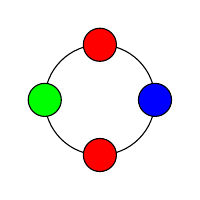
\begin{tikzpicture}[scale=0.7]
\draw[fill=white] (0,0) circle (1);
\draw[fill=red] (0,1) circle (0.3);
\draw[fill=blue] (1,0) circle (0.3);
\draw[fill=red] (0,-1) circle (0.3);
\draw[fill=green] (-1,0) circle (0.3);
\end{tikzpicture}
\end{center}
kanssa symmetriset helminauhat ovat seuraavat:
\begin{center}
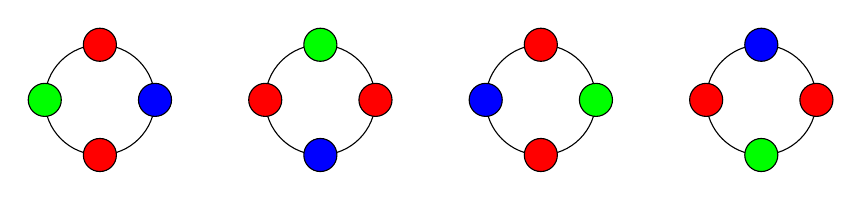
\begin{tikzpicture}[scale=0.7]
\draw[fill=white] (0,0) circle (1);
\draw[fill=red] (0,1) circle (0.3);
\draw[fill=blue] (1,0) circle (0.3);
\draw[fill=red] (0,-1) circle (0.3);
\draw[fill=green] (-1,0) circle (0.3);

\draw[fill=white] (4,0) circle (1);
\draw[fill=green] (4+0,1) circle (0.3);
\draw[fill=red] (4+1,0) circle (0.3);
\draw[fill=blue] (4+0,-1) circle (0.3);
\draw[fill=red] (4+-1,0) circle (0.3);

\draw[fill=white] (8,0) circle (1);
\draw[fill=red] (8+0,1) circle (0.3);
\draw[fill=green] (8+1,0) circle (0.3);
\draw[fill=red] (8+0,-1) circle (0.3);
\draw[fill=blue] (8+-1,0) circle (0.3);

\draw[fill=white] (12,0) circle (1);
\draw[fill=blue] (12+0,1) circle (0.3);
\draw[fill=red] (12+1,0) circle (0.3);
\draw[fill=green] (12+0,-1) circle (0.3);
\draw[fill=red] (12+-1,0) circle (0.3);
\end{tikzpicture}
\end{center}
Tapoja muuttaa asentoa on $n$,
koska helminauhaa voi pyörittää $0,1,\ldots,n-1$
askelta myötäpäivään.
Jos helminauhaa pyörittää 0 askelta,
kaikki $m^n$ väritystä säilyvät ennallaan.
Jos taas helminauhaa pyörittää 1 askeleen,
vain $m$ yksiväristä helminauhaa säilyy ennallaan.

Yleisemmin kun helminauhaa pyörittää $k$ askelta,
ennallaan säilyvien yhdistelmien määrä on
\[m^{\textrm{syt}(k,n)},\]
missä $\textrm{syt}(k,n)$ on lukujen $k$ ja $n$
suurin yhteinen tekijä.
Tämä johtuu siitä, että $\textrm{syt}(k,n)$-kokoiset
pätkät helmiä siirtyvät toistensa paikoille
$k$ askelta eteenpäin.
Niinpä helminauhojen määrä on
Burnsiden lemman mukaan
\[\sum_{i=0}^{n-1} \frac{m^{\textrm{syt}(i,n)}}{n}. \]
Esimerkiksi kun helminauhan pituus on 4
ja värejä on 3, helminauhoja on
\[\frac{3^4+3+3^2+3}{4} = 24. \]

\section{Cayleyn kaava}

Cayleyn kaavan mukaan $n$ solmusta voi
muodostaa $n^{n-2}$ numeroitua puuta.
Puun solmut on numeroitu $1,2,\ldots,n$,
ja kaksi puuta ovat erilaiset,
jos niiden rakenne on erilainen
tai niissä on eri numerointi.

Esimerkiksi kun $n=4$, numeroitujen puiden määrä on $4^{4-2}=16$:

\begin{center}
\begin{tikzpicture}[scale=0.9]
\newcommand\puua[6]{
\path[draw,thick,-] (#1,#2) -- (#1-1.25,#2-1.5);
\path[draw,thick,-] (#1,#2) -- (#1,#2-1.5);
\path[draw,thick,-] (#1,#2) -- (#1+1.25,#2-1.5);
\node[draw, circle, fill=white] at (#1,#2) {#3};
\node[draw, circle, fill=white] at (#1-1.25,#2-1.5) {#4};
\node[draw, circle, fill=white] at (#1,#2-1.5) {#5};
\node[draw, circle, fill=white] at (#1+1.25,#2-1.5) {#6};
}
\newcommand\puub[6]{
\path[draw,thick,-] (#1,#2) -- (#1+1,#2);
\path[draw,thick,-] (#1+1,#2) -- (#1+2,#2);
\path[draw,thick,-] (#1+2,#2) -- (#1+3,#2);
\node[draw, circle, fill=white] at (#1,#2) {#3};
\node[draw, circle, fill=white] at (#1+1,#2) {#4};
\node[draw, circle, fill=white] at (#1+2,#2) {#5};
\node[draw, circle, fill=white] at (#1+3,#2) {#6};
}

\puua{0}{0}{1}{2}{3}{4}
\puua{4}{0}{2}{1}{3}{4}
\puua{8}{0}{3}{1}{2}{4}
\puua{12}{0}{4}{1}{2}{3}

\puub{0}{-3}{1}{2}{3}{4}
\puub{4.5}{-3}{1}{2}{4}{3}
\puub{9}{-3}{1}{3}{2}{4}
\puub{0}{-4.5}{1}{3}{4}{2}
\puub{4.5}{-4.5}{1}{4}{2}{3}
\puub{9}{-4.5}{1}{4}{3}{2}
\puub{0}{-6}{2}{1}{3}{4}
\puub{4.5}{-6}{2}{1}{4}{3}
\puub{9}{-6}{2}{3}{1}{4}
\puub{0}{-7.5}{2}{4}{1}{3}
\puub{4.5}{-7.5}{3}{1}{2}{4}
\puub{9}{-7.5}{3}{2}{1}{4}
\end{tikzpicture}
\end{center}

Seuraavaksi näemme, miten Cayleyn kaavan
voi perustella samastamalla numeroidut puut
Prüfer-koodeihin.

\subsubsection{Prüfer-koodi}

Prüfer-koodi on $n-2$ luvun jono,
joka kuvaa numeroidun puun rakenteen.
Koodi muodostuu poistamalla puusta
joka askeleella lehden, jonka numero on pienin,
ja lisäämällä lehden vieressä olevan solmun
numeron koodiin.

Tarkastellaan esimerkiksi seuraavaa puuta:

\begin{center}
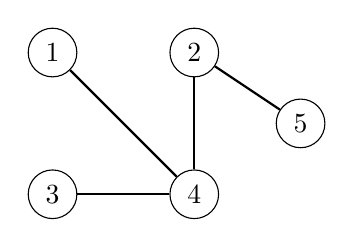
\begin{tikzpicture}[scale=0.9]
\node[draw, circle] (1) at (2,3) {$1$};
\node[draw, circle] (2) at (4,3) {$2$};
\node[draw, circle] (3) at (2,1) {$3$};
\node[draw, circle] (4) at (4,1) {$4$};
\node[draw, circle] (5) at (5.5,2) {$5$};

%\path[draw,thick,-] (1) -- (2);
%\path[draw,thick,-] (1) -- (3);
\path[draw,thick,-] (1) -- (4);
\path[draw,thick,-] (3) -- (4);
\path[draw,thick,-] (2) -- (4);
\path[draw,thick,-] (2) -- (5);
%\path[draw,thick,-] (4) -- (5);
\end{tikzpicture}
\end{center}
Tämän puun Prüfer-koodi on $(4,4,2)$,
koska puusta poistetaan ensin solmu 1,
sitten solmu 3 ja lopuksi solmu 5.

Jokaiselle puulle voidaan laskea
Prüfer-koodi, minkä lisäksi
Prüfer-koodista pystyy palauttamaan
yksikäsitteisesti alkuperäisen puun.
Niinpä numeroituja puita on yhtä monta
kuin Prüfer-koodeja eli $n^{n-2}$.